\begin{figure}[htbp]
\centering
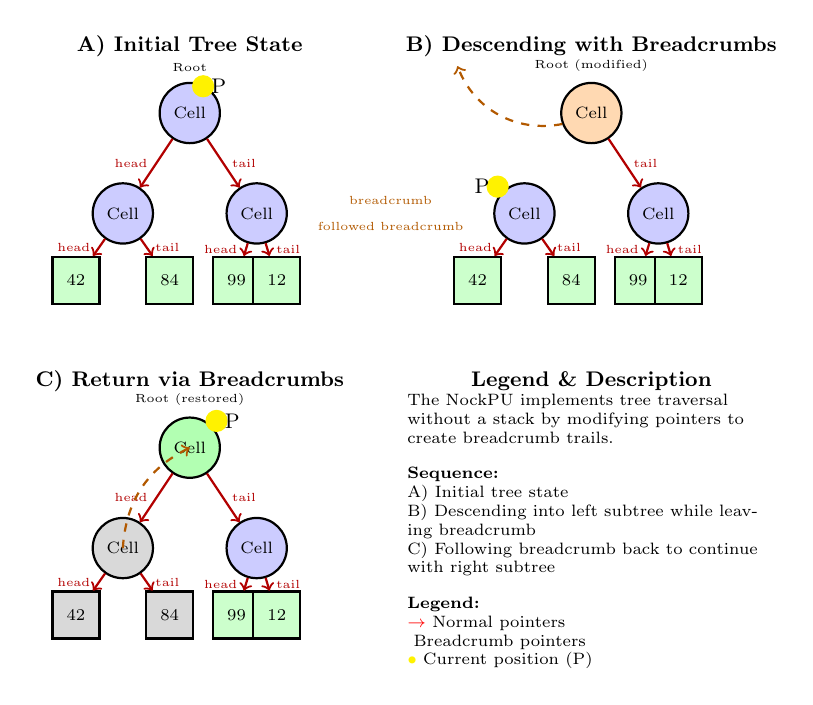
\begin{tikzpicture}[
    scale=0.85,
    transform shape,
    cell/.style={circle, draw=black, thick, fill=blue!20, minimum size=0.9cm, font=\scriptsize},
    atom/.style={rectangle, draw=black, thick, fill=green!20, minimum size=0.7cm, font=\scriptsize},
    pointer/.style={->, thick, red!70!black},
    breadcrumb/.style={->, thick, orange!70!black, dashed},
    label/.style={font=\tiny, above}
]

% Panel A: Initial tree state (top left)
\node[font=\small\bfseries] at (-3, 2.5) {A) Initial Tree State};

% Root cell
\node[cell] (root-a) at (-3, 1.5) {Cell};
\node[label] at (-3, 2) {Root};

% Left subtree
\node[cell] (left-a) at (-4, 0) {Cell};
\node[atom] (left-atom-a) at (-4.7, -1) {42};
\node[atom] (right-atom-a) at (-3.3, -1) {84};

% Right subtree  
\node[cell] (right-a) at (-2, 0) {Cell};
\node[atom] (right-left-a) at (-2.3, -1) {99};
\node[atom] (right-right-a) at (-1.7, -1) {12};

% Initial pointers
\draw[pointer] (root-a) -- (left-a) node[midway, left] {\tiny head};
\draw[pointer] (root-a) -- (right-a) node[midway, right] {\tiny tail};
\draw[pointer] (left-a) -- (left-atom-a) node[midway, left] {\tiny head};
\draw[pointer] (left-a) -- (right-atom-a) node[midway, right] {\tiny tail};
\draw[pointer] (right-a) -- (right-left-a) node[midway, left] {\tiny head};
\draw[pointer] (right-a) -- (right-right-a) node[midway, right] {\tiny tail};

% Current position indicator
\node[fill=yellow, circle, minimum size=0.25cm] at (-2.8, 1.9) {};
\node[right] at (-2.8, 1.9) {\small P};

% Panel B: Traversal down with pointer modifications (top right)
\node[font=\small\bfseries] at (3, 2.5) {B) Descending with Breadcrumbs};

% Root cell (modified)
\node[cell, fill=orange!30] (root-b) at (3, 1.5) {Cell};
\node[label] at (3, 2) {Root (modified)};

% Left subtree
\node[cell] (left-b) at (2, 0) {Cell};
\node[atom] (left-atom-b) at (1.3, -1) {42};
\node[atom] (right-atom-b) at (2.7, -1) {84};

% Right subtree  
\node[cell] (right-b) at (4, 0) {Cell};
\node[atom] (right-left-b) at (3.7, -1) {99};
\node[atom] (right-right-b) at (4.3, -1) {12};

% Modified pointers (breadcrumb in root)
\draw[breadcrumb] (root-b) to[bend left=40] (1, 2.2) node[midway, above] {\tiny breadcrumb};
\draw[pointer] (root-b) -- (right-b) node[midway, right] {\tiny tail};
\draw[pointer] (left-b) -- (left-atom-b) node[midway, left] {\tiny head};
\draw[pointer] (left-b) -- (right-atom-b) node[midway, right] {\tiny tail};
\draw[pointer] (right-b) -- (right-left-b) node[midway, left] {\tiny head};
\draw[pointer] (right-b) -- (right-right-b) node[midway, right] {\tiny tail};

% Current position indicator (moved to left)
\node[fill=yellow, circle, minimum size=0.25cm] at (1.6, 0.4) {};
\node[left] at (1.6, 0.4) {\small P};

% Panel C: Return traversal using breadcrumbs (bottom left)
\node[font=\small\bfseries] at (-3, -2.5) {C) Return via Breadcrumbs};

% Root cell (restored)
\node[cell, fill=green!30] (root-c) at (-3, -3.5) {Cell};
\node[label] at (-3, -3) {Root (restored)};

% Left subtree (visited)
\node[cell, fill=gray!30] (left-c) at (-4, -5) {Cell};
\node[atom, fill=gray!30] (left-atom-c) at (-4.7, -6) {42};
\node[atom, fill=gray!30] (right-atom-c) at (-3.3, -6) {84};

% Right subtree  
\node[cell] (right-c) at (-2, -5) {Cell};
\node[atom] (right-left-c) at (-2.3, -6) {99};
\node[atom] (right-right-c) at (-1.7, -6) {12};

% Restored pointers
\draw[pointer] (root-c) -- (left-c) node[midway, left] {\tiny head};
\draw[pointer] (root-c) -- (right-c) node[midway, right] {\tiny tail};
\draw[pointer] (left-c) -- (left-atom-c) node[midway, left] {\tiny head};
\draw[pointer] (left-c) -- (right-atom-c) node[midway, right] {\tiny tail};
\draw[pointer] (right-c) -- (right-left-c) node[midway, left] {\tiny head};
\draw[pointer] (right-c) -- (right-right-c) node[midway, right] {\tiny tail};

% Breadcrumb trail indicator
\draw[breadcrumb] (-4, -5) to[bend left=30] (-3, -3.5) node[midway, below] {\tiny followed breadcrumb};

% Current position indicator (back at root, ready for right subtree)
\node[fill=yellow, circle, minimum size=0.25cm] at (-2.6, -3.1) {};
\node[right] at (-2.6, -3.1) {\small P};

% Panel D: Caption and Legend (bottom right)
\node[font=\small\bfseries] at (3, -2.5) {Legend \& Description};

\node[text width=5.5cm, font=\scriptsize, align=left] at (3, -4.5) {
\\[0.4cm]
The NockPU implements tree traversal without a stack by modifying pointers to create breadcrumb trails.\\[0.25cm]

\textbf{Sequence:}\\
A) Initial tree state\\
B) Descending into left subtree while leaving breadcrumb\\
C) Following breadcrumb back to continue with right subtree\\[0.25cm]

\textbf{Legend:}\\
\textcolor{red}{$\rightarrow$} Normal pointers \\
\textcolor{orange}{$\dashrightarrow$} Breadcrumb pointers \\
\textcolor{yellow}{$\bullet$} Current position (P) \\
};

\end{tikzpicture}
\caption{Stackless Tree Traversal Sequence demonstrating breadcrumb-based navigation without a traditional call stack.}
\label{fig:tree-traversal}
\end{figure}
